\documentclass{standalone}
\usepackage{tikz}
\usepackage{pgfplots}
\usepgfplotslibrary{groupplots}
\pgfplotsset{compat=1.17}

\begin{document}
	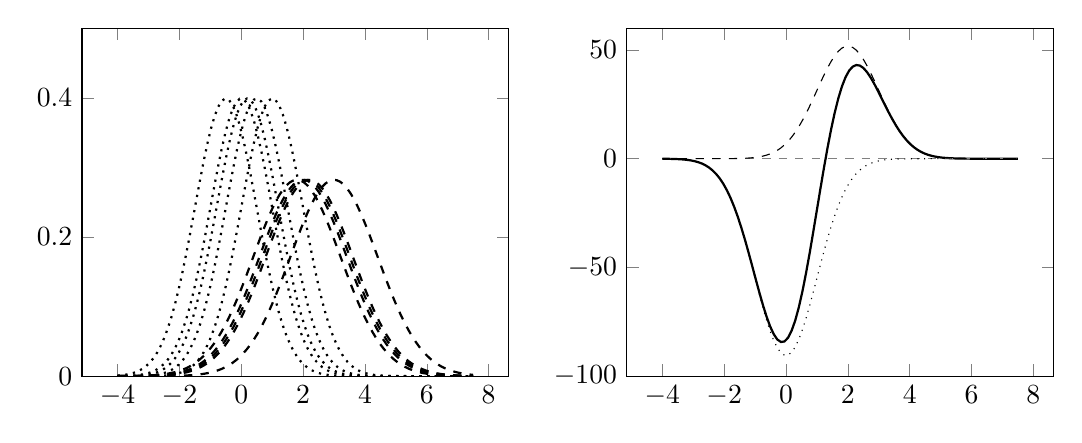
\begin{tikzpicture}
		\begin{groupplot}[
			group style={group size=2 by 1, horizontal sep=1.5cm},
			width=7cm, height=6cm,
			domain=-4:7.5, samples=100,
			axis lines=box,
			ymin=0, ymax=0.5,
			legend style={at={(0.5,1.15)}, anchor=south}
			]
			
			% --- LEFT: Class A, B densities ---
			\nextgroupplot[
			]
			
			% Class A
			\addplot[thick, dotted] {1/(sqrt(2*pi*1)) * exp(-((x - 0)^2) / 2)};
			\addplot[thick, dotted]{1/(sqrt(2*pi*1)) * exp(-((x - 0.5)^2) / 2)};
			\addplot[thick, dotted] {1/(sqrt(2*pi*1)) * exp(-((x - 1)^2) / 2)};
			\addplot[thick, dotted] {1/(sqrt(2*pi*1)) * exp(-((x - 0.2)^2) / 2)};
			\addplot[thick, dotted]{1/(sqrt(2*pi*1)) * exp(-((x + 0.5)^2) / 2)};
			
			% Class B
			\addplot[thick, dashed] {1/(sqrt(2*pi*2)) * exp(-((x - 2)^2) / 4)};
			\addplot[thick, dashed] {1/(sqrt(2*pi*2)) * exp(-((x - 2.1)^2) / 4)};
			\addplot[thick, dashed] {1/(sqrt(2*pi*2)) * exp(-((x - 3)^2) / 4)};
			\addplot[thick, dashed] {1/(sqrt(2*pi*2)) * exp(-((x - 2.2)^2) / 4)};
			\addplot[thick, dashed] {1/(sqrt(2*pi*2)) * exp(-((x - 1.8)^2) / 4)};
			
			% --- RIGHT: Estimated beta(x) ---
			\nextgroupplot[
			ymin=-100, ymax=60
			]
			
			% Tổng beta(x)
			\addplot[thick, black] {-90.48 * exp(-((x - 0)^2) / 2) + 51.79 * exp(-((x - 2)^2) / 2)};
			
			% Zero line
			\addplot[gray, dashed] {0};
			
			% Thành phần basis
			\addplot[dotted] {-90.48 * exp(-((x - 0)^2) / 2)};
			
			\addplot[dashed] {51.79 * exp(-((x - 2)^2) / 2)};
						
		\end{groupplot}
	\end{tikzpicture}
\end{document}
